\documentclass{beamer}
\beamertemplatenavigationsymbolsempty
\setbeamertemplate{footline}[frame number]
\setbeamertemplate{caption}[numbered]
\usetheme{default}
\usecolortheme[named=purple]{structure}

\usepackage[utf,nonfrench,finemath]{kotex}
% 한글 처리를 위한 패키지

\usepackage{graphicx}
% 이미지를 넣기 위한 패키지

\usepackage{wrapfig}
% 이미지 위치 조정 가능

\usepackage{grffile}
\usepackage{amsmath, amsfonts, amsthm, amssymb} % Math packages
\usepackage{braket, dsfont, times}
\usepackage{pgffor}
\usepackage{verbatim}

\usepackage{anyfontsize}

%Information to be included in the title page:
\title{DQN visualization}
\author{Minyoung Jeong}
\institute{Yonsei Univ.}
\date{2023. 01. 13.}

\begin{document}

\begin{frame}
    \titlepage
\end{frame}


% new page

\begin{frame}{Initial condition}

    \hfill \break
    {\fontsize{12}{0} \selectfont SIR model}
    % {\fontsize{size}{baselineskip} \selectfont content}
    \hfill \break

    \; {\fontsize{9}{20} \selectfont max time: 30}
    \hfill \break

    \; {\fontsize{9}{20} \selectfont epsilon start: 1}

    \; {\fontsize{9}{20} \selectfont epsilon decay: 0.995}
    
    \; {\fontsize{9}{20} \selectfont epsilon end: 0.001}
    \hfill \break

    \; {\fontsize{9}{20} \selectfont S0: 9990}

    \; {\fontsize{9}{20} \selectfont I0: 10}

    \; {\fontsize{9}{20} \selectfont gamma: 0.5}
    \hfill \break

    \; {\fontsize{9}{20} \selectfont beta: 0.0005, 0.0010}
    \hfill \break

    \; {\fontsize{9}{20} \selectfont nu: 0.1, 0.2}
    \hfill \break


\end{frame}



\begin{frame}{S, I, Vaccination}
    \foreach \beta in {5, 10}{
        \begin{figure}[tb]
            \includegraphics[width=0.4\textwidth]{images/nu10beta\beta/SIR_w_vac_2000.png}
            \includegraphics[width=0.4\textwidth]{images/nu20beta\beta/SIR_w_vac_2000.png}
        \end{figure}
    }
\end{frame}

\begin{frame}{S, I, Vaccination}
    \foreach \beta in {5, 10}{
        \begin{figure}[tb]
            \includegraphics[width=0.4\textwidth]{images/nu10beta\beta/value_initial.png}
            \includegraphics[width=0.4\textwidth]{images/nu20beta\beta/value_initial.png}
        \end{figure}
    }
\end{frame}

\begin{frame}{S, I, Vaccination}
    \foreach \beta in {5, 10}{
        \begin{figure}[tb]
            \includegraphics[width=0.4\textwidth]{images/nu10beta\beta/value_2000.png}
            \includegraphics[width=0.4\textwidth]{images/nu20beta\beta/value_2000.png}
        \end{figure}
    }
\end{frame}


% % Case 1

% \foreach beta in {1000, 2000, 4000, 8000, 16000} {
%     \begin{frame}{Case 1\_ Learning result}
        
%         {\fontsize{10}{50} \selectfont After \n \, episodes learning:}

%         \begin{figure}[tb]
%             \includegraphics[height=0.5\textheight]{../발표 자료/\n_result.png}
%         \end{figure}
%     \end{frame}

%     \begin{frame}{Case 1\_ Learning result}

%         \begin{figure}[tb]
%             \includegraphics[height=0.4\textheight]{../발표 자료/\n_action.png}
%             \includegraphics[height=0.4\textheight]{../발표 자료/\n_value.png}
%         \end{figure}

%     \end{frame}
% }


% % new page

% \begin{frame}{Case 2}

%     \begin{wrapfigure}{R}{0.5\textwidth}
%         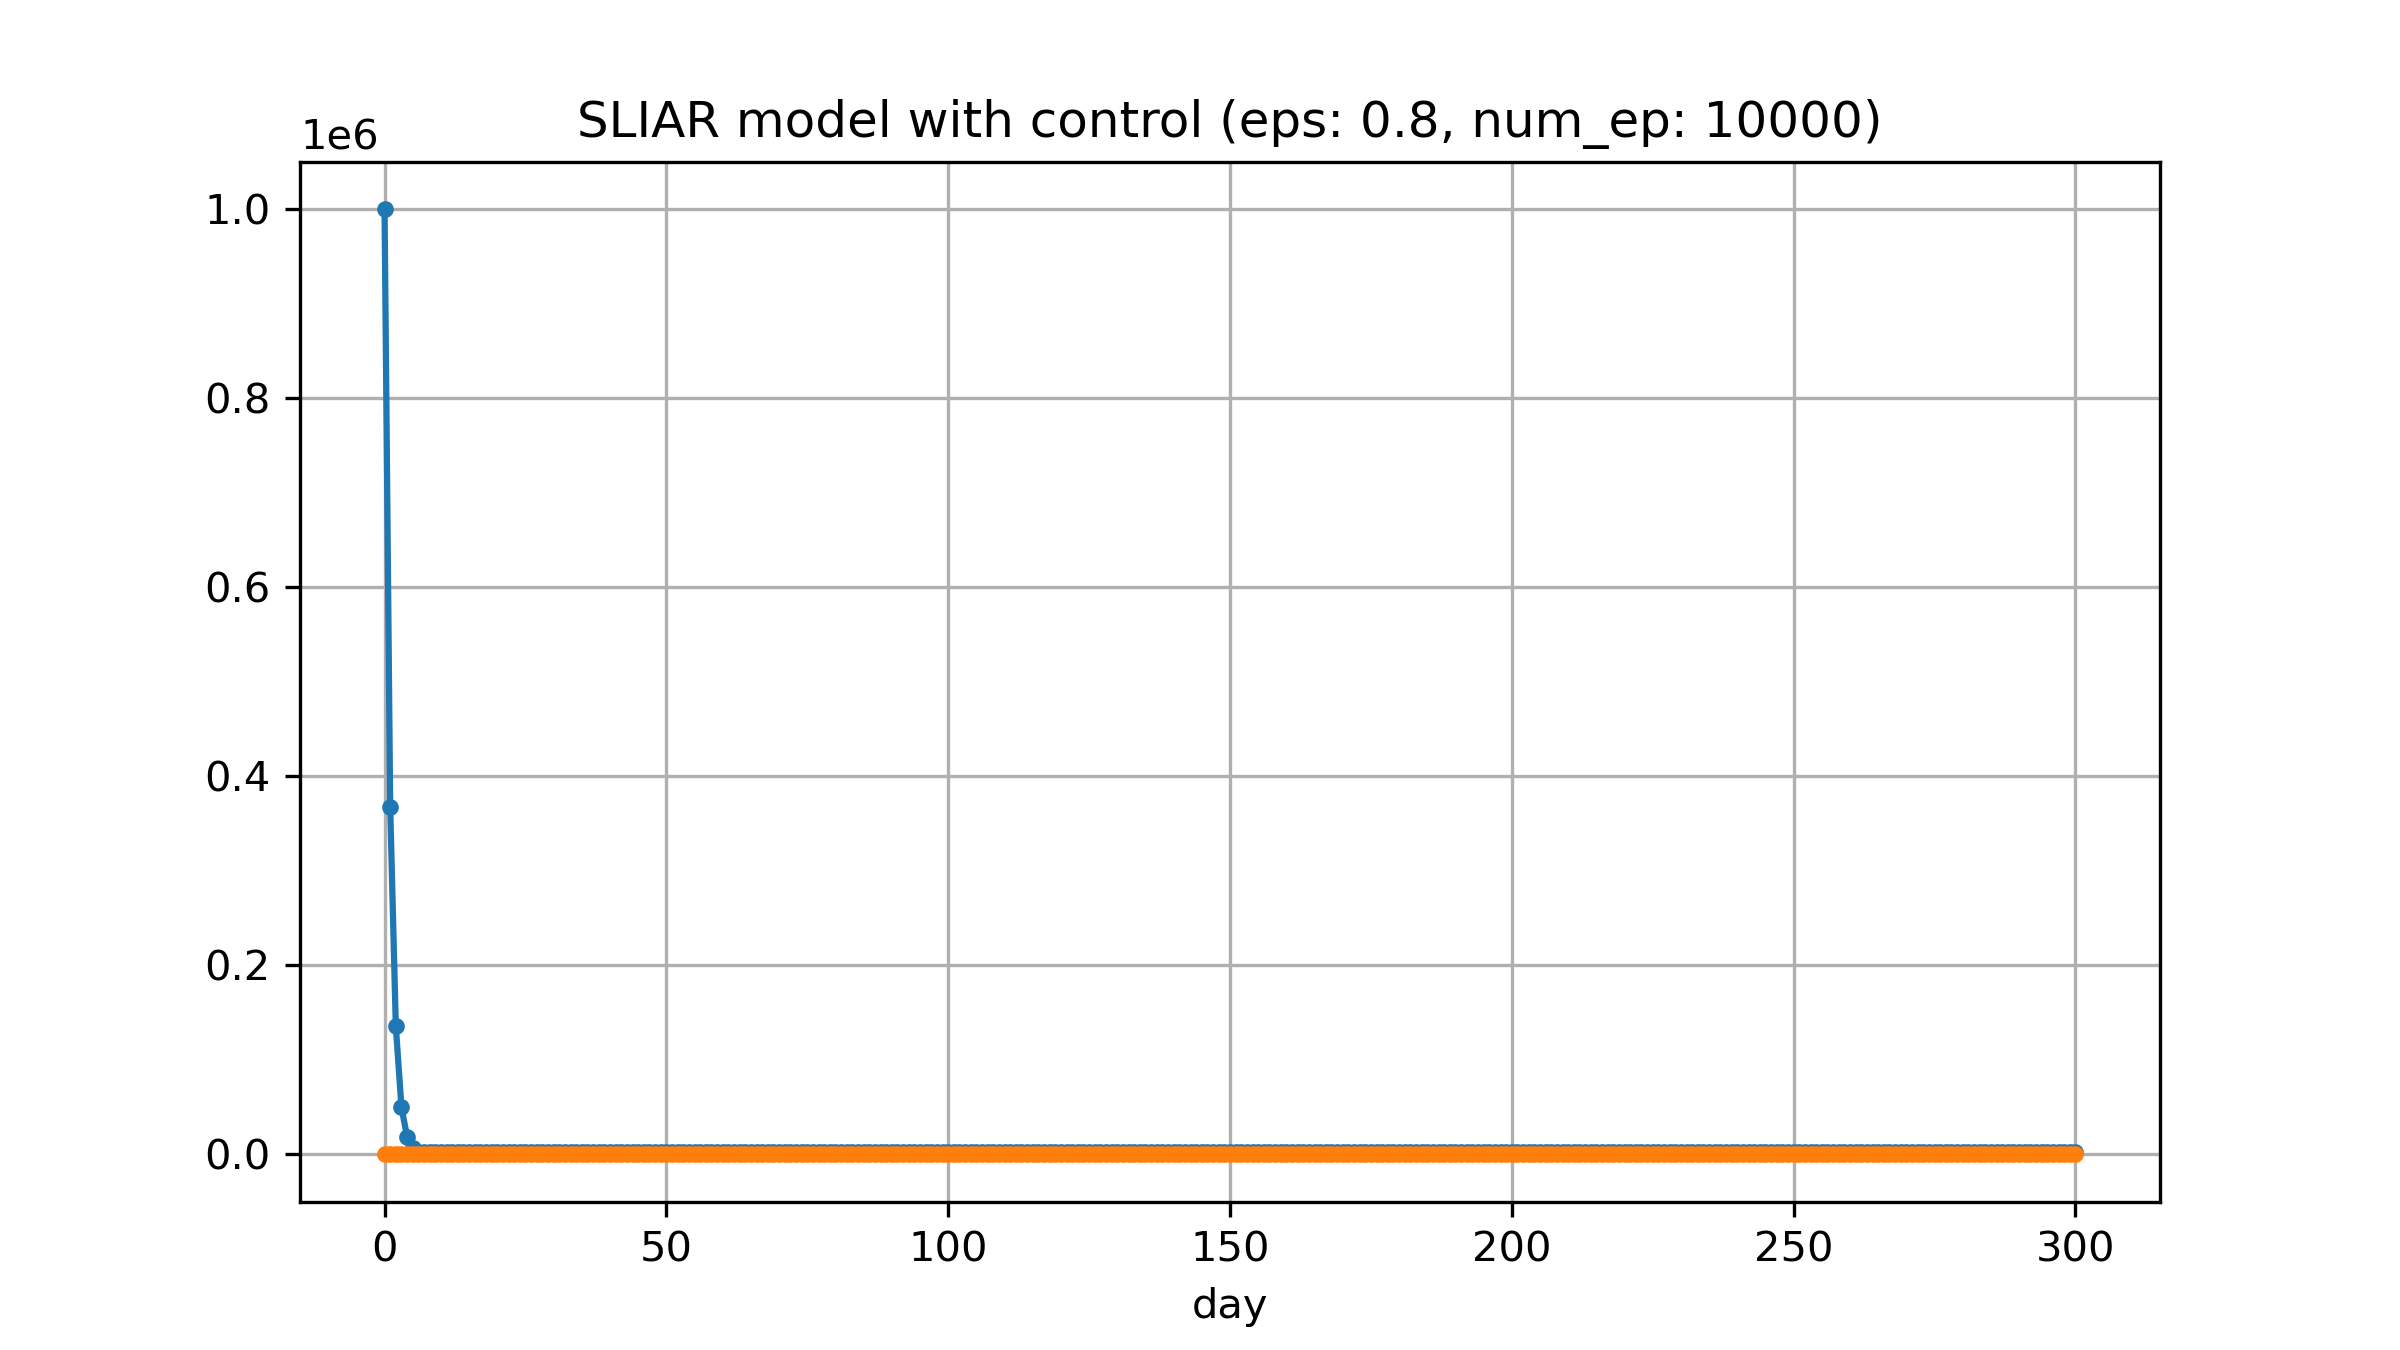
\includegraphics[width=0.48\textwidth]{../발표 자료/SLIAR_w_control_0.8,10000.png}
%         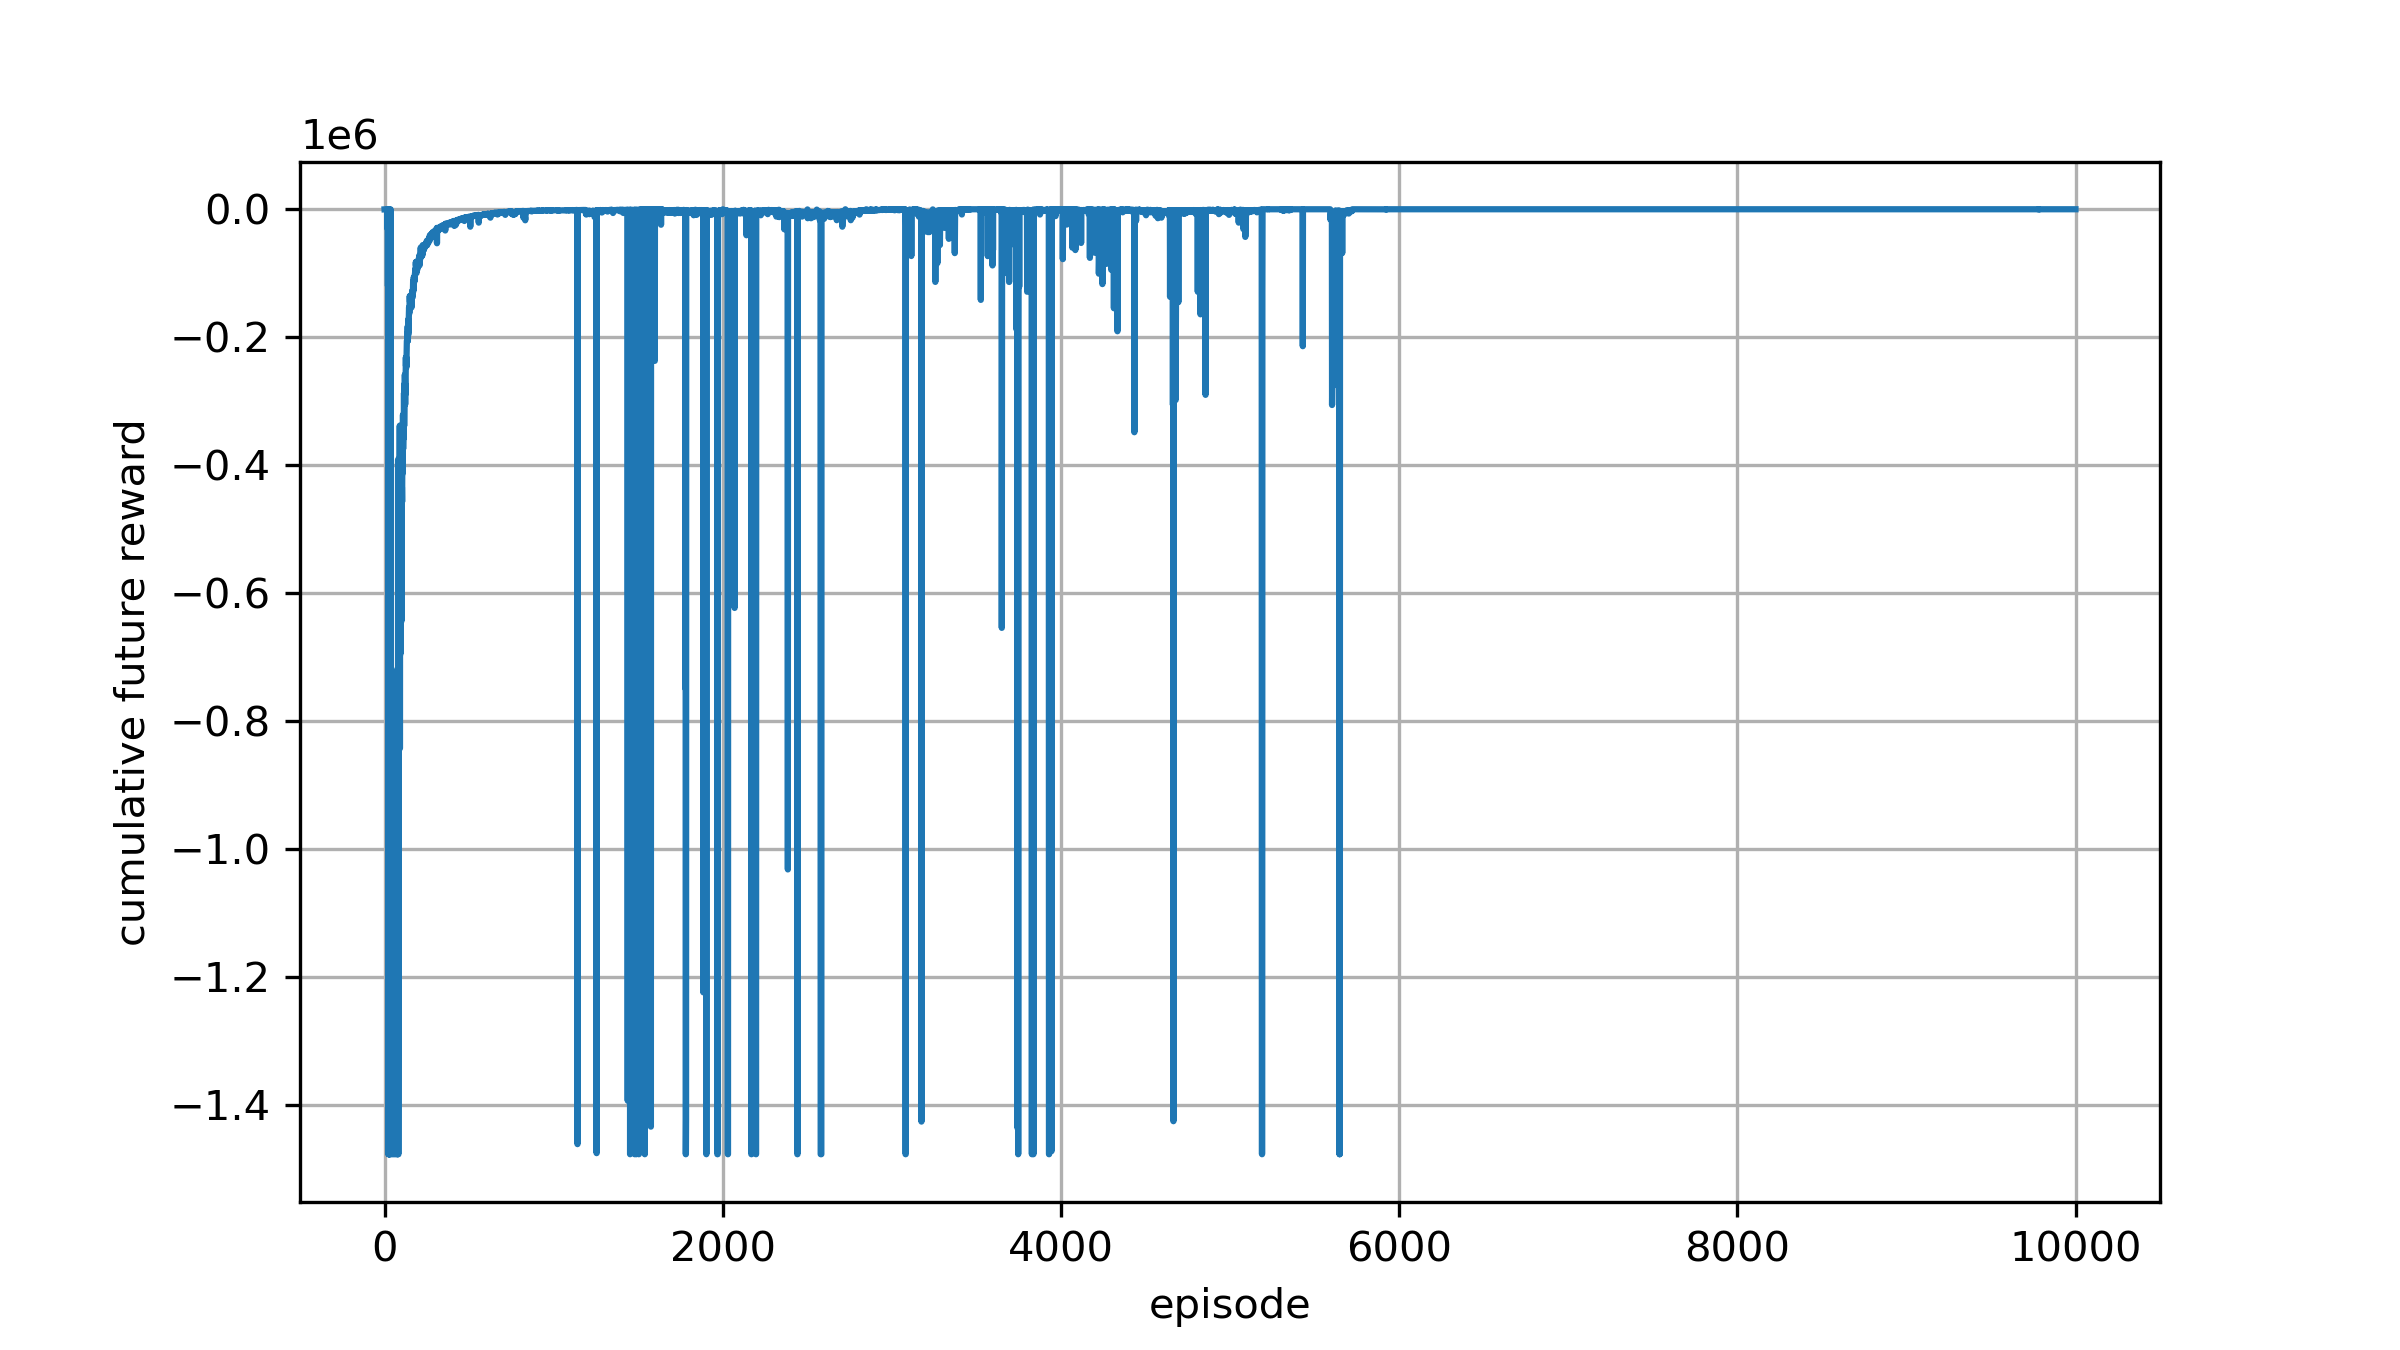
\includegraphics[width=0.48\textwidth]{../발표 자료/SLIAR_score_0.8,10000.png}
%     \end{wrapfigure}

%     {\fontsize{15}{50} \selectfont Initial}
%     % {\fontsize{size}{baselineskip} \selectfont content}
%     \hfill \break
%     \hfill \break

%     \; max time: 300
%     \hfill \break

%     \; epsilon start: 1
%     \hfill \break

%     \; epsilon decay: 0.8

% \end{frame}


% % Case 2

% \foreach \n in {1000, 2000, 4000, 8000, 12000} {
%     \begin{frame}{Case 2\_ Learning result}
        
%         {\fontsize{10}{50} \selectfont After \n \, episodes learning:}

%         \begin{figure}[tb]
%             \includegraphics[height=0.5\textheight]{../발표 자료/80decay_\n_result.png}
%         \end{figure}
%     \end{frame}

%     \begin{frame}{Case 2\_ Learning result}

%         \begin{figure}[tb]
%             \includegraphics[height=0.4\textheight]{../발표 자료/80decay_\n_action.png}
%             \includegraphics[height=0.4\textheight]{../발표 자료/80decay_\n_value.png}
%         \end{figure}

%     \end{frame}
% }



\end{document}